\normaltrue \difficilefalse \tdifficilefalse
\correctiontrue

%\UPSTIidClasse{11} % 11 sup, 12 spé
%\newcommand{\UPSTIidClasse}{12}

\exer{Parallélépipède percé$\star$ \label{B2:10:41}}
\setcounter{question}{0}\UPSTIcompetence[2]{B2-10}
\index{Compétence B2-10}
\index{Parallélépipède}
\ifcorrection
\else
\marginnote{\textbf{Pas de corrigé pour cet exercice.}}
\fi

\ifprof
\else
La matrice d'inertie d'un cylindre d'axe $\axe{G}{k}$ de rayon $R$ et de hauteur $H$ et de masse $m$ est donnée en son centre d'inertie par 
$\inertie{G}{1}=\matinertie{A}{A}{C}{0}{0}{0}{\base{i}{j}{k}}$ avec $A=m\left(\dfrac{R^2}{4}+\dfrac{H^2}{12} \right)$ et $C=m\dfrac{R^2}{2}$. 


La matrice d'inertie d'un parallélépipède rectangle de cotés $a$, $b$ et $c$ et de masse $m$ est donnée en son centre d'inertie par 
$\inertie{G}{1}=\matinertie{A}{B}{C}{0}{0}{0}{\base{i}{j}{k}}$ avec $A={m\dfrac{b^2+c^2}{12}}$, $B={m\dfrac{a^2+c^2}{12}}$, $C={m\dfrac{a^2+b^2}{12}}$.

Soit la pièce suivante. 
\begin{figure}[H]
\centering
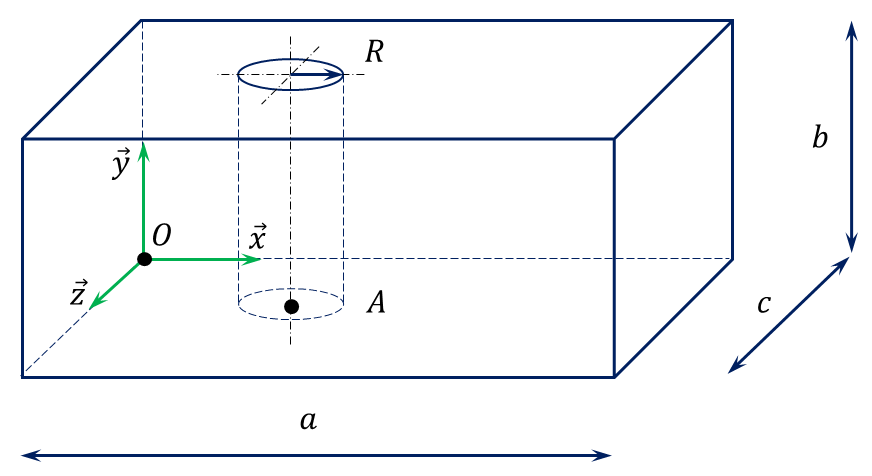
\includegraphics[width=\linewidth]{41_01}
\end{figure}

On pose $\vect{OA}=\dfrac{a}{3}\vect{x}+\dfrac{c}{2}\vect{z}$. 

\fi



\question{Déterminer la position du centre d'inertie $G$ du solide.}
\ifprof
On note $m_C$ la masse du cylindre (plein) et $m_P$ la masse du parallélépipède. On a alors $m=m_P-m_C$.
De plus, $\vect{OG_P}=\dfrac{a}{2}\vect{x}+\dfrac{b}{2}\vect{y}+\dfrac{c}{2}\vect{z}$
et $\vect{OG_C}=\dfrac{a}{3}\vect{x}+\dfrac{b}{2}\vect{y}+\dfrac{c}{2}\vect{z}$.

On a alors 
$m \vect{OG}=m_P \vect{OG_P}-m_C \vect{OG_C} = m_P \left(\dfrac{a}{2}\vect{x}+\dfrac{b}{2}\vect{y}+\dfrac{c}{2}\vect{z} \right)-m_C \left( \dfrac{a}{3}\vect{x}+\dfrac{b}{2}\vect{y}+\dfrac{c}{2}\vect{z}\right) $.

Par suite, 
$\vect{OG}=
\begin{pmatrix}
x_G \\ y_G \\ z_G
\end{pmatrix}_{\base{x}{y}{z}}
=
\begin{pmatrix}
\dfrac{a}{m_P-m_C} \left( \dfrac{m_P}{2} -  \dfrac{m_C}{3}\right) \\
b/2 \\
c/2
\end{pmatrix}_{\base{x}{y}{z}}
$.
\else
\fi

\question{Déterminer la matrice d'inertie du solide en $G$.}
\ifprof ~\\

Les plans $(G,\vect{x},\vect{y})$ et $(G,\vect{z},\vect{x})$ sont des plans de symétrie. 
On a donc $\inertie{G}{S}=\matinertie{A}{B}{C}{0}{0}{0}{\mathcal{B}}$.

\textbf{On déplace la matrice du parallélépipède rectangle en G.}

On a $\inertie{G_P}{P}=\matinertie{A_P}{B_P}{C_P}{0}{0}{0}{\mathcal{B}}$ et


$\vect{G_P G} = \vect{G_P O} + \vect{O G} = 
\begin{pmatrix}
-\dfrac{a}{2} \\
-\dfrac{b}{2} \\
-\dfrac{c}{2}
\end{pmatrix}_{\mathcal{B}} 
+
\begin{pmatrix}
\dfrac{a}{m_P-m_C} \left( \dfrac{m_P}{2} -  \dfrac{m_C}{3}\right) \\
b/2 \\
c/2
\end{pmatrix}_{\mathcal{B}}=
\begin{pmatrix}
\dfrac{a}{m_P-m_C} \left( \dfrac{m_P}{2} -  \dfrac{m_C}{3}\right) -\dfrac{a}{2}\\
0 \\
0
\end{pmatrix}_{\mathcal{B}}=
\begin{pmatrix}
\Delta_x\\
0 \\
0
\end{pmatrix}_{\mathcal{B}}$.

Ainsi, 
$\inertie{G}{P} = \inertie{G_P}{P} + m_P\begin{pmatrix}
0 & 0 & 0\\
0 & \Delta_x^2 & 0 \\
0 & 0 & \Delta_x^2
\end{pmatrix}_{\mathcal{B}}
= \matinertie{A_P}{B_P+m_P\Delta_x^2}{C_P+m_P\Delta_x^2}{0}{0}{0}{\mathcal{B}}
$

\textbf{On déplace la matrice du cylindre en G.}

De même $\inertie{G_C}{C}=\matinertie{A_C}{B_C}{A_C}{0}{0}{0}{\mathcal{B}}$ et

$\vect{G_C G} = \vect{G_C O} + \vect{O G} = 
\begin{pmatrix}
-\dfrac{a}{3} \\
-\dfrac{b}{2} \\
-\dfrac{c}{2}
\end{pmatrix}_{\mathcal{B}} 
+
\begin{pmatrix}
\dfrac{a}{m} \left( \dfrac{m_P}{2} -  \dfrac{m_C}{3}\right) \\
b/2 \\
c/2
\end{pmatrix}_{\mathcal{B}}=
\begin{pmatrix}
\dfrac{a}{m} \left( \dfrac{m_P}{2} -  \dfrac{m_C}{3}\right) -\dfrac{a}{3}\\
0 \\
0
\end{pmatrix}_{\mathcal{B}}=
\begin{pmatrix}
\Delta_x'\\
0 \\
0
\end{pmatrix}_{\mathcal{B}}$.

Ainsi, 
$\inertie{G}{C} = \inertie{G_C}{C} + m_C\begin{pmatrix}
0 & 0 & 0\\
0 & \Delta_x'^2 & 0 \\
0 & 0 & \Delta_x'^2
\end{pmatrix}_{\mathcal{B}}
= \matinertie{A_C}{B_C+m_C\Delta_x'^2}{A_C+m_C\Delta_x'^2}{0}{0}{0}{\mathcal{B}}
$.

\textbf{Bilan.}

Au final, $\inertie{G}{E} = \inertie{G}{P} - \inertie{G}{C}$ et 

$\inertie{G}{E} = \matinertie{A_P-A_C}{B_P+m_P\Delta_x^2-B_C-m_C\Delta_x'^2}{C_P+m_P\Delta_x^2-A_C-m_C\Delta_x'^2}{0}{0}{0}{\mathcal{B}} $

%Notons (1) le parallélépipède rectangle et (2) le cylindre (plein). On note $\mathcal{B}_0=\base{x}{y}{z}$
%On a $\inertie{G}{1}=\matinertie{A_1}{B_1}{C_1}{0}{0}{0}{\mathcal{B}_0}$ et
%$\inertie{G}{2}=\matinertie{A_2}{B_2}{A_2}{0}{0}{0}{\mathcal{B}_0}$ (attention l'axe du cylindre est $\vect{y}$).
%
%On a donc $\inertie{G}{S}=\matinertie{A_1-A_2}{B_1-B_2}{C_1-A_2}{0}{0}{0}{\mathcal{B}_0}$.
%
%Par ailleurs, $m=m_1-m_2$
%et $\vect{AG}=\dfrac{b}{2}\vect{y}$; donc $\inertie{A}{S}=\matinertie{A_1-A_2+m\dfrac{b^2}{4}}{B_1-B_2}{C_1-A_2+m\dfrac{b^2}{4}}{0}{0}{0}{\mathcal{B}_0}$.
%
%Enfin, $\vect{OG}=\dfrac{a}{2}\vect{x}+\dfrac{b}{2}\vect{y}+\dfrac{c}{2}\vect{z}$; donc
% $\inertie{O}{S}=
%\matinertie{A_1-A_2}{B_1-B_2}{C_1-A_2}{0}{0}{0}{\mathcal{B}_0}
%+m\matinertie{\dfrac{b^2}{4}+\dfrac{c^2}{4}}{\dfrac{a^2}{4}+\dfrac{c^2}{4}}{\dfrac{a^2}{4}+\dfrac{b^2}{4}}{-\dfrac{bc}{4}}{-\dfrac{ac}{4}}{-\dfrac{ab}{4}}{\mathcal{B}_0}$.
\else
\fi


\ifprof
\else
\begin{flushright}
\footnotesize{Corrigé voir \ref{B2:10:41}.}
\end{flushright}%
\fi